\documentclass[]{article}
\usepackage{lmodern}
\usepackage{amssymb,amsmath}
\usepackage{ifxetex,ifluatex}
\usepackage{fixltx2e} % provides \textsubscript
\ifnum 0\ifxetex 1\fi\ifluatex 1\fi=0 % if pdftex
  \usepackage[T1]{fontenc}
  \usepackage[utf8]{inputenc}
\else % if luatex or xelatex
  \ifxetex
    \usepackage{mathspec}
  \else
    \usepackage{fontspec}
  \fi
  \defaultfontfeatures{Ligatures=TeX,Scale=MatchLowercase}
\fi
% use upquote if available, for straight quotes in verbatim environments
\IfFileExists{upquote.sty}{\usepackage{upquote}}{}
% use microtype if available
\IfFileExists{microtype.sty}{%
\usepackage{microtype}
\UseMicrotypeSet[protrusion]{basicmath} % disable protrusion for tt fonts
}{}
\usepackage[margin=1in]{geometry}
\usepackage{hyperref}
\PassOptionsToPackage{usenames,dvipsnames}{color} % color is loaded by hyperref
\hypersetup{unicode=true,
            pdftitle={Revised Proposal},
            pdfauthor={Group A - Felix Stetsenko, Enoch Shin},
            colorlinks=true,
            linkcolor=Maroon,
            citecolor=Blue,
            urlcolor=blue,
            breaklinks=true}
\urlstyle{same}  % don't use monospace font for urls
\usepackage{color}
\usepackage{fancyvrb}
\newcommand{\VerbBar}{|}
\newcommand{\VERB}{\Verb[commandchars=\\\{\}]}
\DefineVerbatimEnvironment{Highlighting}{Verbatim}{commandchars=\\\{\}}
% Add ',fontsize=\small' for more characters per line
\usepackage{framed}
\definecolor{shadecolor}{RGB}{248,248,248}
\newenvironment{Shaded}{\begin{snugshade}}{\end{snugshade}}
\newcommand{\AlertTok}[1]{\textcolor[rgb]{0.94,0.16,0.16}{#1}}
\newcommand{\AnnotationTok}[1]{\textcolor[rgb]{0.56,0.35,0.01}{\textbf{\textit{#1}}}}
\newcommand{\AttributeTok}[1]{\textcolor[rgb]{0.77,0.63,0.00}{#1}}
\newcommand{\BaseNTok}[1]{\textcolor[rgb]{0.00,0.00,0.81}{#1}}
\newcommand{\BuiltInTok}[1]{#1}
\newcommand{\CharTok}[1]{\textcolor[rgb]{0.31,0.60,0.02}{#1}}
\newcommand{\CommentTok}[1]{\textcolor[rgb]{0.56,0.35,0.01}{\textit{#1}}}
\newcommand{\CommentVarTok}[1]{\textcolor[rgb]{0.56,0.35,0.01}{\textbf{\textit{#1}}}}
\newcommand{\ConstantTok}[1]{\textcolor[rgb]{0.00,0.00,0.00}{#1}}
\newcommand{\ControlFlowTok}[1]{\textcolor[rgb]{0.13,0.29,0.53}{\textbf{#1}}}
\newcommand{\DataTypeTok}[1]{\textcolor[rgb]{0.13,0.29,0.53}{#1}}
\newcommand{\DecValTok}[1]{\textcolor[rgb]{0.00,0.00,0.81}{#1}}
\newcommand{\DocumentationTok}[1]{\textcolor[rgb]{0.56,0.35,0.01}{\textbf{\textit{#1}}}}
\newcommand{\ErrorTok}[1]{\textcolor[rgb]{0.64,0.00,0.00}{\textbf{#1}}}
\newcommand{\ExtensionTok}[1]{#1}
\newcommand{\FloatTok}[1]{\textcolor[rgb]{0.00,0.00,0.81}{#1}}
\newcommand{\FunctionTok}[1]{\textcolor[rgb]{0.00,0.00,0.00}{#1}}
\newcommand{\ImportTok}[1]{#1}
\newcommand{\InformationTok}[1]{\textcolor[rgb]{0.56,0.35,0.01}{\textbf{\textit{#1}}}}
\newcommand{\KeywordTok}[1]{\textcolor[rgb]{0.13,0.29,0.53}{\textbf{#1}}}
\newcommand{\NormalTok}[1]{#1}
\newcommand{\OperatorTok}[1]{\textcolor[rgb]{0.81,0.36,0.00}{\textbf{#1}}}
\newcommand{\OtherTok}[1]{\textcolor[rgb]{0.56,0.35,0.01}{#1}}
\newcommand{\PreprocessorTok}[1]{\textcolor[rgb]{0.56,0.35,0.01}{\textit{#1}}}
\newcommand{\RegionMarkerTok}[1]{#1}
\newcommand{\SpecialCharTok}[1]{\textcolor[rgb]{0.00,0.00,0.00}{#1}}
\newcommand{\SpecialStringTok}[1]{\textcolor[rgb]{0.31,0.60,0.02}{#1}}
\newcommand{\StringTok}[1]{\textcolor[rgb]{0.31,0.60,0.02}{#1}}
\newcommand{\VariableTok}[1]{\textcolor[rgb]{0.00,0.00,0.00}{#1}}
\newcommand{\VerbatimStringTok}[1]{\textcolor[rgb]{0.31,0.60,0.02}{#1}}
\newcommand{\WarningTok}[1]{\textcolor[rgb]{0.56,0.35,0.01}{\textbf{\textit{#1}}}}
\usepackage{graphicx,grffile}
\makeatletter
\def\maxwidth{\ifdim\Gin@nat@width>\linewidth\linewidth\else\Gin@nat@width\fi}
\def\maxheight{\ifdim\Gin@nat@height>\textheight\textheight\else\Gin@nat@height\fi}
\makeatother
% Scale images if necessary, so that they will not overflow the page
% margins by default, and it is still possible to overwrite the defaults
% using explicit options in \includegraphics[width, height, ...]{}
\setkeys{Gin}{width=\maxwidth,height=\maxheight,keepaspectratio}
\IfFileExists{parskip.sty}{%
\usepackage{parskip}
}{% else
\setlength{\parindent}{0pt}
\setlength{\parskip}{6pt plus 2pt minus 1pt}
}
\setlength{\emergencystretch}{3em}  % prevent overfull lines
\providecommand{\tightlist}{%
  \setlength{\itemsep}{0pt}\setlength{\parskip}{0pt}}
\setcounter{secnumdepth}{0}
% Redefines (sub)paragraphs to behave more like sections
\ifx\paragraph\undefined\else
\let\oldparagraph\paragraph
\renewcommand{\paragraph}[1]{\oldparagraph{#1}\mbox{}}
\fi
\ifx\subparagraph\undefined\else
\let\oldsubparagraph\subparagraph
\renewcommand{\subparagraph}[1]{\oldsubparagraph{#1}\mbox{}}
\fi

%%% Use protect on footnotes to avoid problems with footnotes in titles
\let\rmarkdownfootnote\footnote%
\def\footnote{\protect\rmarkdownfootnote}

%%% Change title format to be more compact
\usepackage{titling}

% Create subtitle command for use in maketitle
\providecommand{\subtitle}[1]{
  \posttitle{
    \begin{center}\large#1\end{center}
    }
}

\setlength{\droptitle}{-2em}

  \title{Revised Proposal}
    \pretitle{\vspace{\droptitle}\centering\huge}
  \posttitle{\par}
    \author{Group A - Felix Stetsenko, Enoch Shin}
    \preauthor{\centering\large\emph}
  \postauthor{\par}
      \predate{\centering\large\emph}
  \postdate{\par}
    \date{November 12, 2019}


\begin{document}
\maketitle

\begin{enumerate}
\def\labelenumi{\arabic{enumi}.}
\item
  \textbf{Group:} A
\item
  \textbf{Group Members:} Enoch Shin and Felix Stetsenko
\item
  \textbf{Title:} \emph{Visualizing Transportation Network Provider and
  Taxi trips in Chicago}
\item
  \textbf{Purpose:} Our initial idea is to visualize travel patterns
  across the City of Chicago using Transportation Network Provider (TNPs
  referring to rideshare companies like Uber and Lyft) and Taxi trip
  data publicly available on Chicago's Data Portal website. We would
  visualize the origins and destinations (on the census tract level) of
  all taxi and TNP trips across the city from November 2018 to present.
  We could then use the data visualization for a number of possible
  analyses:

  \begin{itemize}
  \item
    Do TNP and taxi services serve the same market, or is one service
    preferred over the other for certain travel markets (e.g.~trips
    originating from O'Hare Airport)?
  \item
    Can residential segregation be visualized through TNP and taxi
    service and trip patterns? For instance, is there a relationship
    between census tract demographics and TNP vs.~taxi share of trips
    originating from that census tract?
  \item
    Using a clustering algorithm on the origin / destination data, how
    closely would the clusters reflect neighborhood boundaries and
    racial and socio-economic divides?
  \end{itemize}
\end{enumerate}

\hypertarget{data-overview}{%
\section{5. Data Overview}\label{data-overview}}

\textbf{Data:} The relevant data is all publicly available, either from
the City of Chicago or the U.S. Census Bureau. We would create a
visualization by using an overlay on top of the Google Maps API. We
would consider adding the functionality to have the data continuously
update as the City of Chicago posts updates on its Data Portal.

\hypertarget{variables}{%
\section{6. Variables}\label{variables}}

\hypertarget{transportation-network-provider-data}{%
\subsection{Transportation Network Provider
Data}\label{transportation-network-provider-data}}

\begin{quote}
A TNP company is defined by the City of Chicago as a ``ride share
company, which provides prearranged transportation services for
compensation through an Internet-enabled application or digital platform
connecting passengers with drivers of vehicles for hire. TNP drivers and
their vehicles join and become affiliated with TNP companies and are
then available to be dispatched through the TNP's digital platform. Each
TNP company must be licensed. The TNP license is an annual license which
is not transferable.''
\end{quote}

\begin{quote}
Link: City of Chicago TNP data (available from November 2018 to
present):
\url{https://data.cityofchicago.org/Transportation/Transportation-Network-Providers-Trips/m6dm-c72p}
\end{quote}

\hypertarget{codebook-chicago-tnp-data-available-from-november-2018-to-present}{%
\subsection{Codebook: Chicago TNP data (available from November 2018 to
present)}\label{codebook-chicago-tnp-data-available-from-november-2018-to-present}}

Trip ID

\begin{quote}
A unique identifier for the trip
\end{quote}

Trip Start Timestamp

\begin{quote}
When the trip started, rounded to the nearest 15 minutes (floating
timestamp).
\end{quote}

Trip End Timestamp

\begin{quote}
When the trip ended, rounded to the nearest 15 minutes (floating
timestamp).
\end{quote}

Trip Seconds

\begin{quote}
Time of the trip in seconds.
\end{quote}

Trip Miles

\begin{quote}
Distance of the trip in miles.
\end{quote}

Pickup Census Tract

\begin{quote}
The Census Tract where the trip began.
\end{quote}

Dropoff Census Tract

\begin{quote}
The Census Tract where the trip ended.
\end{quote}

Pickup Community Area

\begin{quote}
The Community Area where the trip began.
\end{quote}

Dropoff Community Area

\begin{quote}
The Community Area where the trip ended.
\end{quote}

Fare

\begin{quote}
The fare for the trip, rounded to the nearest \$2.50.
\end{quote}

Tip

\begin{quote}
The tip for the trip, rounded to the nearest \$1.00.
\end{quote}

Additional Charges

\begin{quote}
The taxes, fees, and any other charges for the trip (dollars).
\end{quote}

Trip Total

\begin{quote}
Total cost of the trip (dollars).
\end{quote}

Shared Trip Authorized

\begin{quote}
Whether the customer agreed to a shared trip with another passenger.
\end{quote}

Trips Pooled

\begin{quote}
If customers were matched for a shared trip, how many trips, including
this one, were pooled.
\end{quote}

Pickup Centroid Latitude

\begin{quote}
The latitude of the center of the pickup census tract.
\end{quote}

Pickup Centroid Longitude

\begin{quote}
The longitude of the center of the pickup census tract.
\end{quote}

Pickup Centroid Location

\begin{quote}
The location of the center of the pickup census tract.
\end{quote}

Dropoff Centroid Latitude

\begin{quote}
The latitude of the center of the dropoff census tract.
\end{quote}

Dropoff Centroid Longitude

\begin{quote}
The longitude of the center of the dropoff census tract.
\end{quote}

Dropoff Centroid Location

\begin{quote}
The location of the center of the dropoff census tract.
\end{quote}

\hypertarget{taxi-data}{%
\subsection{Taxi Data}\label{taxi-data}}

\begin{quote}
Link: City of Chicago Taxi data (available from 2013 to present):
\url{https://data.cityofchicago.org/Transportation/Taxi-Trips/wrvz-psew}
\end{quote}

\begin{quote}
City of Chicago Taxi data (available from 2013 to present)
\end{quote}

Trip ID

\begin{quote}
A unique identifier for the trip.
\end{quote}

Taxi ID

\begin{quote}
A unique identifier for the taxi.
\end{quote}

Trip Start Timestamp

\begin{quote}
When the trip started, rounded to the nearest 15 minutes.
\end{quote}

Trip End Timestamp

\begin{quote}
When the trip ended, rounded to the nearest 15 minutes.
\end{quote}

Trip Seconds

\begin{quote}
Time of the trip in seconds.
\end{quote}

Trip Miles

\begin{quote}
Distance of the trip in miles.
\end{quote}

Pickup Census Tract

\begin{quote}
The Census Tract where the trip began.
\end{quote}

Dropoff Census Tract

\begin{quote}
The Census Tract where the trip ended.
\end{quote}

Pickup Community Area

\begin{quote}
The Community Area where the trip began.
\end{quote}

Dropoff Community Area

\begin{quote}
The Community Area where the trip ended.
\end{quote}

Fare

\begin{quote}
The fare for the trip.
\end{quote}

\hypertarget{demographic-data-from-census-bureau-and-national-historical-gis-work-in-progress}{%
\subsection{Demographic Data from Census Bureau and National Historical
GIS (Work in
Progress)}\label{demographic-data-from-census-bureau-and-national-historical-gis-work-in-progress}}

\begin{quote}
Link: 2017 American Community Survey 5-year Estimates Subject Tables
(available at the census tract level):
\url{https://data.census.gov/cedsci/map?table=B00001\&tid=ACSDT5Y2017.B00001\&hidePreview=false\&vintage=2017\&layer=censustract\&cid=B00001_001E\&lastDisplayedRow=34}
\end{quote}

\begin{quote}
Link 2: \url{https://www.nhgis.org/} for shapefiles with race
\end{quote}

\begin{quote}
We'll not include a detailed codebook since we're not sure if it'll be
plausible to use this data, for the following reasons below:
\end{quote}

\begin{quote}
The Census Bureau data appears to lack geographic information about race
distribution (i.e.~the data tells us summaries of counts of racial
groups, but it's unclear if the Bureau releases the general locations of
these demographics). The goal of the project is to see if there are any
patterns in rideshare usage that are associated with racial
distributions, so we're interested in demographic data.
\end{quote}

\begin{quote}
The National Historical GIS data is more inline with what we're looking
for, but we cannot query this data with an API: we have to go through
the site and put in a request for the data through their portal, and
then they send a notification via email that the data is ready to
download. Turnaround only takes a couple minutes, though. However, the
University of Virginia has already detailed their process for mapping
distributions of demographic groups (link
\href{https://demographics.coopercenter.org/racial-dot-map\#thedata}{here}),
and it seems like an entire project of its own. I presume we can find a
way of adapting the University's code to our project, but I also think
we should put limits on the scope of this project since we're already
working with large quantities of data with the TNP data set.
\end{quote}

\hypertarget{end-product}{%
\section{7. End Product}\label{end-product}}

The final deliverable will be an interactive, animated visualization
overlaid over the Google Maps API; it will show Taxi and TNP trips for a
few selected days from the data set (selected from November 2018 to
present).* The user will have the option of selecting specific time
frames, origin / destination census tracts, and adding additional layers
to the map (e.g.~public transit lines, demographic and socio-economic
variables).

*At the moment, we are focusing on a specific holiday (Valentine's Day:
February 14, 2019), and two specific days (Saturday, February 2, 2019;
Monday, February 4, 2018) for analysis. We may have to adjust the scope
(i.e.~make it on the order of several hours instead of a day). However,
the actual querying with the API is mostly sorted out.

\hypertarget{sample-of-the-data}{%
\subsection{Sample of the Data}\label{sample-of-the-data}}

Below, we've just done a simple query of the TNP data with data from
Valentine's Day 2019.No other particular filters or constraints were
done for the query. However, see our \texttt{chicagoIngest.Rmd} file to
view our progress on navigating the API.

\hypertarget{ingest-query}{%
\section{Ingest (Query)}\label{ingest-query}}

\begin{quote}
City of Chicago data uses the Socrata API.
\end{quote}

\begin{Shaded}
\begin{Highlighting}[]
\NormalTok{url <-}\StringTok{ "https://data.cityofchicago.org/resource/m6dm-c72p.json"}
\CommentTok{# names <- readRDS("ChicagoCommute/names.Rda")}
\NormalTok{mytoken <-}\StringTok{ "bJZzO3D3YpmgVEszO9oq241gH"}
\end{Highlighting}
\end{Shaded}

\begin{Shaded}
\begin{Highlighting}[]
\CommentTok{# valday <- read.socrata(paste0(url, "?","$where=trip_start_timestamp between '2019-02-14T00:00:00' and '2019-02-14T23:59:59'"),  app_token=mytoken)}
\CommentTok{# saveRDS(valday, "ChicagoCommute/RDA/valday.Rda")}
\NormalTok{valday <-}\StringTok{ }\KeywordTok{readRDS}\NormalTok{(}\StringTok{"ChicagoCommute/RDA/valday.Rda"}\NormalTok{)}
\end{Highlighting}
\end{Shaded}

\hypertarget{wrangle}{%
\section{Wrangle}\label{wrangle}}

\begin{Shaded}
\begin{Highlighting}[]
\CommentTok{# toCoord <- grep(".coordinates$", names(valday), value = TRUE)}
\CommentTok{# val_coord <- valday %>%}
              \CommentTok{# rowwise() %>%}
              \CommentTok{# mutate_at(.funs=function(x)\{paste(unlist(x), collapse=",")\}, }
                        \CommentTok{# toCoord)}
\NormalTok{toNum <-}\StringTok{ }\KeywordTok{c}\NormalTok{(}\StringTok{"trip_seconds"}\NormalTok{, }\StringTok{"trip_miles"}\NormalTok{, }\StringTok{"fare"}\NormalTok{, }\StringTok{"tip"}\NormalTok{,}
          \StringTok{"additional_charges"}\NormalTok{, }\StringTok{"trip_total"}\NormalTok{)}

\NormalTok{coordNum <-}\StringTok{ }\KeywordTok{grep}\NormalTok{(}\StringTok{"_centroid_l[[:alpha:]]*e$"}\NormalTok{, }\KeywordTok{names}\NormalTok{(valday), }\DataTypeTok{value=}\OtherTok{TRUE}\NormalTok{)}

\NormalTok{valday <-}\StringTok{ }\NormalTok{valday }\OperatorTok\StringTok{ }
\StringTok{            }\KeywordTok{mutate_at}\NormalTok{(}\DataTypeTok{.funs=}\NormalTok{as.numeric, }\KeywordTok{c}\NormalTok{(toNum, coordNum))}
\end{Highlighting}
\end{Shaded}

\begin{quote}
We need to do a sample of the Valentine's Day dataset since
\textasciitilde315k data points take prohibitively long to plot.
\end{quote}

\begin{Shaded}
\begin{Highlighting}[]
\CommentTok{#quick conversion to numeric for some variables of interest}
\NormalTok{subval <-}\StringTok{ }\NormalTok{mosaic}\OperatorTok{::}\KeywordTok{sample}\NormalTok{(valday, }\DataTypeTok{size=}\DecValTok{2500}\NormalTok{)}
\NormalTok{toNum <-}\StringTok{ }\KeywordTok{c}\NormalTok{(}\StringTok{"pickup_centroid_longitude"}\NormalTok{, }\StringTok{"pickup_centroid_latitude"}\NormalTok{,}
           \StringTok{"dropoff_centroid_longitude"}\NormalTok{, }\StringTok{"dropoff_centroid_latitude"}\NormalTok{)}
\NormalTok{subval }\OperatorTok\StringTok{ }\KeywordTok{mutate_at}\NormalTok{(}\DataTypeTok{.funs=}\NormalTok{as.numeric, toNum)}
        
\KeywordTok{qmplot}\NormalTok{(pickup_centroid_longitude, pickup_centroid_latitude, }
       \DataTypeTok{data =}\NormalTok{ subval, }
       \DataTypeTok{maptype =} \StringTok{"toner-lite"}\NormalTok{, }
       \DataTypeTok{color =} \KeywordTok{I}\NormalTok{(}\StringTok{"red"}\NormalTok{))}
\end{Highlighting}
\end{Shaded}

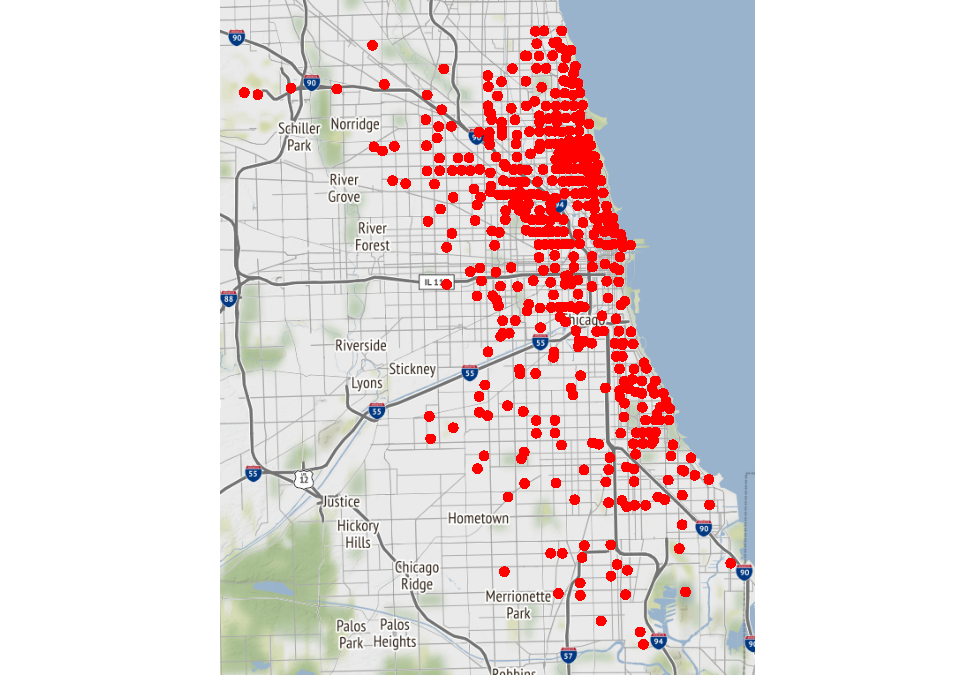
\includegraphics{RevisedProposal_files/figure-latex/unnamed-chunk-4-1.pdf}

\begin{quote}
This shows us the pickup locations for the rideshare records on a
selection of 3,000 queried observations.
\end{quote}

\hypertarget{table-of-head-of-data}{%
\subsection{Table of Head of Data}\label{table-of-head-of-data}}

Quitting from lines 266-267 (RevisedProposal.Rmd) Error in
head(chicago\_df) : object `chicago\_df' not found Calls: \ldots{}
withCallingHandlers -\textgreater{} withVisible -\textgreater{} eval
-\textgreater{} eval -\textgreater{} -\textgreater{} head In addition:
Warning messages: 1: In knitr::knit(knit\_input, knit\_output, envir =
envir, quiet = quiet, : The file ``RevisedProposal.Rmd'' must be encoded
in UTF-8. Please see
\url{https://yihui.name/en/2018/11/biggest-regret-knitr/} for more info.
2: Removed 147 rows containing missing values (geom\_point).


\end{document}
